% todo: q5, q2.1
\documentclass[11pt,onecolumn,letterpaper]{article}
\usepackage{amsmath,amssymb,amsthm,graphicx,xspace,multirow,tikz}
\usetikzlibrary{arrows,automata,shapes}
\usepackage[titlenotnumbered,noend,noline]{algorithm2e}
\usepackage{listings}
\usepackage[compact]{titlesec}
\usepackage{XCharter}
\usepackage[T1]{fontenc}
\usepackage[scaled]{beramono}
\usepackage{multicol}
\usepackage{enumitem}

\tikzstyle{block} = [rectangle, draw, fill=blue!20, 
    text width=5em, text centered, rounded corners, minimum height=2em]
\tikzstyle{bt} = [rectangle, draw, fill=blue!20, 
    text width=4em, text centered, rounded corners, minimum height=2em]
\setlength{\evensidemargin}{-0.1in} \setlength{\oddsidemargin}{-0.1in}
\setlength{\textwidth}{6.5in} \setlength{\textheight}{9.0in}
\setlength{\topmargin}{-0.5in}
\setlength{\parindent}{0in}
\setlength{\parskip}{0.125in}

\newcounter{qNum}
\setcounter{qNum}{1}
%\newcommand{\q}[1]{\vspace*{0.10in} \noindent
%\arabic{qNum}.~(#1)\stepcounter{qNum}}
\newcommand{\q}[1]{%\vspace*{0.10in} \noindent
\textbf{(#1)}\stepcounter{qNum}}

\newcommand*\circled[1]{\tikz[baseline=(char.base)]{
    \node[shape=circle,draw,inner sep=2pt] (char) {#1};}}
    
\lstset{basicstyle=\footnotesize\ttfamily,breaklines=true}

\newcommand{\solpara}{\vspace*{0.0625in}\noindent\textbf{Solution}\hspace*{0.25in}}

\title{SE 465 W19 Final Solutions}
\author{Patrick Lam}

\begin{document}
\vspace{-12em}

\maketitle

\q{1a} Many acceptable answers. Structured input is the key. 1) We
could use hierarchical fuzzing for any Unix-like utility that accepts
input. Simple levels of the hierarchy could just pass in random
characters, while higher ones could provide valid input that is
somehow interesting (e.g.  input is very long, or has an interesting
combination of option flags). 2) Word processor import functionality.
3) Media players. etc.

\q{1b} Sample answer:
FindBugs. False positives can occur for any static rule violation that
is for some reason deliberately left in the codebase. These can include
things like unreachable code and unhandled exceptions.

More generally, false positives come from considering impossible
executions. There is an abstraction and if the abstraction can't
differentiate between a false positive and a true positive, then
the tool can report a false positive. For instance, say an error
condition only trips if a value is negative, but that value
is computed by squaring some input (and hence is always positive).

\q{1c} Sample answer: AddressSanitizer (Asan). Asan aborts whenever it encounters a memory
error, so it will miss any cascading memory errors. It is up to the
user to re-run Asan to find any remaining errors.

Another type of answer, and more the one I was hoping for, is
that dynamic analysis will miss anything that requires a particular
input to trigger.

\q{1d} Sample answer: A logical conflict between changes (i.e. changesets C1 and C2
do not have a merge conflict, and both pass tests on their own,
but cause test failures when combined)

Another answer: Forgetting to add a file to the repo, or failing to build under the
specific configuration that CI tests (which may be different from the dev's build environment.)

\q{1e}
Setup: Beginning up to {\tt rules.addRule(rule)};\\
Teardown: None\\
Exercising: The {\tt p.getSourceCodeProcessor()\ldots} line\\
Verifying: The two asserts at the end.

\q{1f}
State. We are using accessor methods to gather information
about the final state of {\tt r}, instead of observing how the state
of {\tt r} came to be (e.g. observing what methods were called).

\q{1g}
Advantages:
\begin{itemize}[noitemsep]
\item Can improve code quality
\item Can communicate valuable lessons to the author and other contributors
\end{itemize}

Disadvantages (as far as I know I never discussed them, so that was the opportunity to think about it a bit on your own):
\begin{itemize}[noitemsep]
\item Takes time and effort (opportunity cost)
\item Bad code reviews can result in lots of back-and-forth over trivial details and bad inter-dev climate.
\end{itemize}

\q{1h} 
Sample answer: Firefox adds "invalid" attribute to image that seems valid.\\
Actual bug summary: Some images gets a spurious "invalid" ATK state attribute, leading to AT technologies to ignore them.\\[1em]

Talking about AT is not mandatory, although it's not a bad idea if you are trying to provide context for why someone might care
about the bug.

\q{1i}
The write to {\tt n->data} succeeded. Some things we can deduce based on this are:
\begin{itemize}[noitemsep]
\item the memory requested by {\tt calloc (sizeof(struct node))} was allocated successfully,
and we are writing to valid memory
\item the node struct has a {\tt data} field compatible with the value 5 (e.g. int, short, etc.)
\end{itemize}

\q{1j}
Levels of test coverage may not be an indicator of the quality of tests. Although we have
CRTC, the tests applied to the round trips may hardly test system behavior at all (e.g. no
asserts in any tests). One thing that could be done to improve tests is to make sure
each test has an assert for important values for each visited state. If we are able to
edit the FSM, another thing we could do is make the states more granular.

\newpage

\q{2.1} (2 points) a) There might be a {\tt NullPointerException}. The open ({\tt
  new Reader}) may throw an {\tt IOException} (FileNotFound), which is
caught; execution then proceeds to the {\tt close} on the null {\tt
  reader}.

b) (5 points) {\tt @Nullable} is not necessary since {\tt readFile()} cannot be called with a null {\tt BufferedReader} from what is seen here. Either the instantiation of {\tt new BufferedReader} will succeed or fail. If it succeeds, then {\tt reader} isn't null. If it fails, then the call to {\tt readFile()} doesn't happen.

@Nullable would be necessary when there is a possibility {\tt BufferedReader r} passed in can be null, e.g. if we may fail to instantiate the 'reader' variable by moving the {\tt readFile} call to after the {\tt catch}. we will then need a null pointer exception check in the function.

c) (3 points) This code will not pass FB Infer, since FB Infer thinks {\tt BufferedReader r} might be null when it enters the function and performing {\tt r.readLine()} on a null {\tt r} will fail. The code should be modified to include a {\tt if (r == null) { return; }} line as the first line in the function.

\q{2.2} One example:

Original Program $p$
\begin{lstlisting}
void threshold(int a, int b)
{
    int result = a+b;
    if (result > 10)
    {
        cout << "threshold not " << endl;
    }
    cout << "OK" << endl;
}
\end{lstlisting}

Mutated Program $m$
\begin{lstlisting}
void threshold(int a, int b)
{
    int result = a+b;
    if (result >= 10) //added =
    {
        cout << "threshold not " << endl;
    }
    cout << "OK" << endl;
}
\end{lstlisting}

Suppose $T: \{ \langle a = 4, b = 6\rangle\}$; the test case should print ``OK''.
The test $T$ achieves statement coverage on $m$ as $a+b=10$ and $4+6>=10$ enters the if block, but does not on $p$ since $4+6>10$ does not enter the if block. I added the = sign to the if block so that running $T$ on $m$ will enter whereas running $T$ on $p$ will not.

My test suite $T$ kills $m$, since running $T$ on $m$ will print ``threshold not OK'' but my test suite will be expecting the run to print ``OK''.

\newpage
\q{3} The clarification was ``edge coverage = branch coverage''. I didn't say that you had to produce a CFG, but you probably should
so that you can be sure that you achieve all of the edges. We wouldn't mark it, but it certainly helps in evaluating your solution.

\begin{center}
\begin{tikzpicture}[->,>=stealth',shorten >=1pt,auto,node distance=1.5cm,
                    semithick,initial text=]

  \node[initial,bt,text width=7em]   (1)                     {1. if len == 6};
  \node[bt,text width=5em]           (2) [below right=1,xshift=1em,yshift=-2.4em]     {2. print(6)};
  \node[bt]           (3) [below left of=2,xshift=-1em,yshift=-.5em]   {3. i = 0};
  \node[bt,text width=7em]           (4) [below of=3] {4. if i < s.len};
  \node[bt,text width=6em]           (5) [below of=4] {5. if isAlpha};
  \node[bt,text width=6em]           (6) [below right of=5,xshift=1em,yshift=-1em] {6. print(r)};
  \node[bt,text width=9em]           (7) [below left of=6,xshift=-1em,yshift=-.5em]   {7. print(charAt(i))};
  \node[bt]           (8) [below of=7] {8. i++};
  \node[bt,text width=5em]           (9) [right of=4,xshift=4em] {9. return};

  \path (1) edge node[yshift=-.5em] {T} (2)
  (1) edge node[left] {F} (3)
  (2) edge node {} (3)
  (3) edge node {} (4)
  (4) edge node {T} (5)
  (4) edge node {F} (9)
  (5) edge node[yshift=-.4em] {T} (6)
  (5) edge node[left] {F} (7)
  (6) edge node {} (7)
  (7) edge node {} (8)
  (4) edge node {} (9)
  (8.west) edge[bend left]  node {} (4.west);
\end{tikzpicture}
\end{center}

Test requirements:
\[ \{ (1, 2), (2, 3), (1, 3), (3, 4), (4, 9), (4, 5), (5, 6), (5, 7), (6, 7), (7, 8), (8, 4) \} \]

Let's take care of the 6 vs. not 6 by including strings "123456" and "1" in the input.

The loop definitely terminates for finite-length strings so we can be sure
that $(4,9)$ is always going to execute. So that really just leaves making sure
that we have an alpha and a non-alpha character in the string.
So adding strings "abc123" and "123" would suffice.

The other edges are unconditionally reached assuming you enter the loop
(i.e. you have an input of strictly positive length).

You could minimize the test suite, but why would you?


\newpage

\q{4a} Oops. A significant minority of the class told me there are four mistakes.
Sorry. You only have to
identify 3 mistakes. And, I changed the mistakes from the ones on the 2017 final.

\begin{itemize}[noitemsep]
\item So, of course, {\tt mockTransport()} fits the definition of a mistake. I meant it to say
{\tt mockTransport}; I didn't mean it to be a mistake.

\item {\tt mockDriver} should be a mock, namely {\tt mock(Driver)}.
\item {\tt setDestination(10)} does not match the destination of {\tt 5} that the {\tt Person} constructor
  is going to set.
\item There is no base price set (so it's actually impossible to say what the payment should be).
\item {\tt waitUntilArrivedAt()} should take a parameter (which should be 100).
\end{itemize}

\q{4b} (2 points for state vs behaviour) That is a state-based assert on the {\tt Person} class. We should use a behaviour-based test to be consistent
with {\tt testGoHome}.

The number 405 also is incorrect somehow. I'm not sure how that happened. 


(3 points for suggesting a fix): mocking Person is not a fix, because then you'd be just testing the test.
Other reasonable suggestions get points. The best fix would modify everything to make the distance travelled
visible through the classes here (e.g. the driver should report that.)

\q{5} (a) A clarification here was that I was just expecting yes-or-no; an answer doesn't have to capture
the declaration itself.

\begin{verbatim}
//LocalVariableDeclaration[count(./VariableDeclarator)>1]
\end{verbatim}

(b) The prompt was just ``Write an XPath expression which detects empty catch blocks''.
This works.
\begin{verbatim}
//CatchStatement/Block[descendant::BlockStatement]
\end{verbatim}
So does this:
\begin{verbatim}
//CatchStatement/Block[count(./BlockStatement)<1]
\end{verbatim}

People responded to the ``expected'' thing, which was fine. Sometimes people started
further up the tree. Let's not dock marks for that, unless it's too far up the tree that
it is unnecessarily restrictive. I expect that many solutions wouldn't actually work, but that's
fine, since students don't have a computer at hand. Just look for the concepts of locating the node and
then filtering on something that seems reasonable.

\q{6} Oops, I forgot some closing statements. Here's what the grammar should look like.

\begin{verbatim}
desc :- building*
building :- "building" BUILDING "\n" floor* "end-building\n"
floor :- "floor" DIGIT "\n" room* "end-floor\n"
room :- "room" DIGIT DIGIT DIGIT DIGIT "\n" occupant* "end-room\n"
occupant :- "occupant" OCCUPANT "\n"
\end{verbatim}

In a context-free grammar it's quite hard to enforce the stated constraint. You could do it at a
grammar level by having a bunch of floorN productions. But that would be weird. Better to do it at a
higher level, for instance by modifying generated rooms so that they meet the stated constraint.

\end{document}
